\section{Numerical Results}
\label{sec:numRes}
We now have some MFT predictions about the SPM, and a few ideas about when those predictions might be invalid. Thus, it is prudent for us to test them out numerically.
There are a few different methods which could have been used, but we chose to calculate using the excellent \texttt{KMCLib}\cite{leetmaa2014kmclib} package, which implements the Kinetic Monte Carlo algorithm (essentially the same as the Gillespie algorithm)
on lattice systems. \texttt{KMCLib} has the advantage that it is python-wrapped \texttt{C++}, and thus quite easy to use whilst at the same time being quite computationally efficient; thus it was fairly easy for us to carry out large numbers
of differently-parametrised serial \texttt{KMCLib} jobs on the \texttt{Eddie3} computing cluster here at Edinburgh. The codes used are kept here~\cite{jHellGitRepo}.

As we have MFT predictions about flow in a block, we can try to simulate that situation using KMC. In the bulk, the transition rates are simply those described in Figure~\ref{fig:rates}. At the boundaries, referred to as the ``top''  and ``bottom''
of the block, there are 2 layers of lattice sites what switch between being full and empty with rates such that the time-averaged occupation can be specified to match the desired boundary conditions; there are then chances for particles to spawn
and despawn with rates depending upon the occupation of these boundary layers. In the end, the intention is that these boundaries should reproduce the effect of having particle reservoirs attached to the ends, which is something we can check for
sanity in the output by inspecting the time-averaged occupations of sites near the boundary. I have used this setup to explore three scenarios, discussed in the following sections. In each of these I refer to a boundary condition configuration
by $(\rho_B, \rho_T)$, with $\rho_B$ and $\rho_T$ being the bottom and top boundary densities respectively.
When we measure flow rate in such a situation, we perform a specified number of Gillespie steps and count the number of particles entering at the top $e_T$, leaving at the top $l_T$, entering at the bottom $e_B$, leaving at the bottom $l_B$,
as well as the Gillespie time interval $T$ that elapses during those steps; we then have an estimate of the overall flow rate $J$ via
\begin{equation}
 J = \frac{e_B-e_T+l_T-l_B}{2T}.
\end{equation}
We can also count the total number of particles in the system in order to measure the average particle density, although we need to make sure that it is correctly time-averaged; in my code this is done by updating a histogram of particle numbers
as the simulation progresses. In each of our calculations, we make the initial configuration by randomly filling the system with particles and vacancies in such a way that the initial density should be $\frac{1}{2}(\rho_T + \rho_B)$, and then
run the system for a specified number of equilibration steps to destroy any initial transients.

\subsection{Varying $\lambda$ with Fixed Boundary Conditions}
The MFT we derived suggests that some kind of transition might occur as $\lambda$ varies, as we go from a steady flow regime to a critically slow flow regime. An easy way to see if this happens is to hold the desired boundary densities constant
whilst changing $\lambda$, and measuring the particle density as well as the mean, variance and skewness of the flow rate. If such a transition does indeed occur, we should expect to see a divergence in one of these moments. I have done this with
4 fairly exemplary sets of boundary conditions as shown in Figure~\ref{fig:lambdaScans}. In each case we used systems of length $64$ (length $32$ gives similar results, so this
is probably big enough), running them for $400000$ Gillispie steps for equilibration followed by $10000$ measurement runs of $1000$ steps interspersed with relaxation runs of $16000$
steps. This way we could gather statistics about flow rates and densities in a well-equilibrated system (if possible) whilst not having to worry too much about temporal autocorrelation effects.
\begin{figure*}[h!]
\vspace{1em}
\caption{\label{fig:lambdaScans} Moments of flow rates and average overall densities observed when varying $\lambda$ with fixed boundary densities $(\rho_B, \rho_T)$: Blue refers to $(\frac{2}{3}, \frac{2}{3})$, yellow to $(\frac{3}{4}, \frac{7}{12})$
(both with average density $\frac{2}{3}$); green to $(\frac{3}{4}, \frac{1}{4})$, red to $(\frac{99}{100}, \frac{1}{100})$ (with average density $\frac{1}{2}$). In the case of the mean flow we have an MFT prediction, indicated by the solid line.}
\begin{center}
 \begin{tabular}{c|c}
    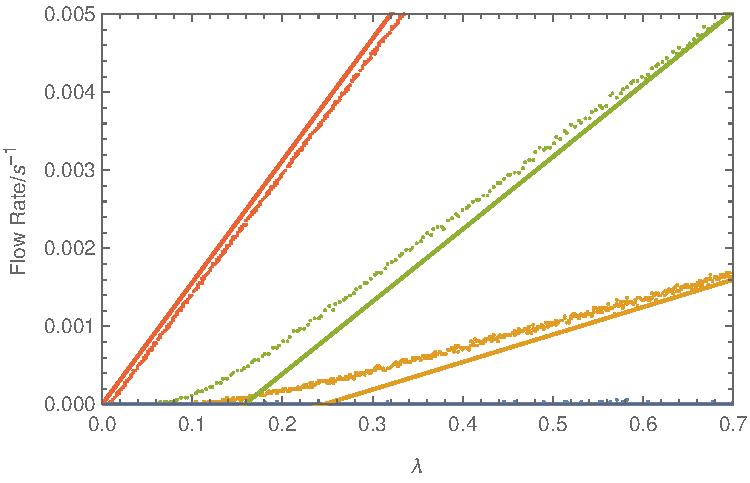
\includegraphics[width=0.5\linewidth]{../tex-src/images/lambdaScan/flowMean} & 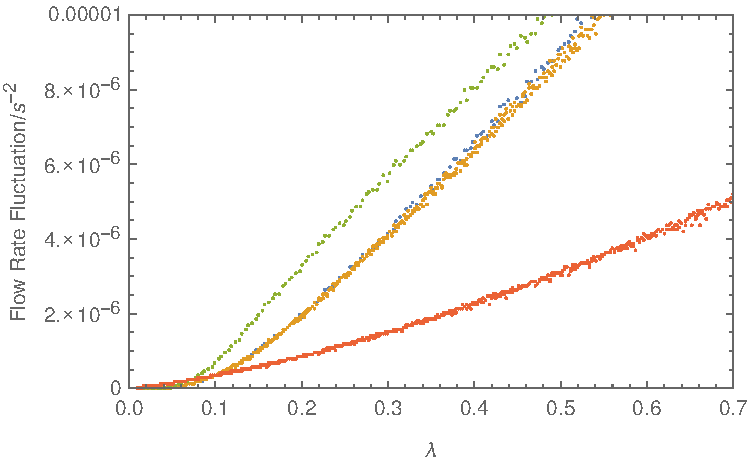
\includegraphics[width=0.5\linewidth]{../tex-src/images/lambdaScan/flowVar} \\
    \hline
    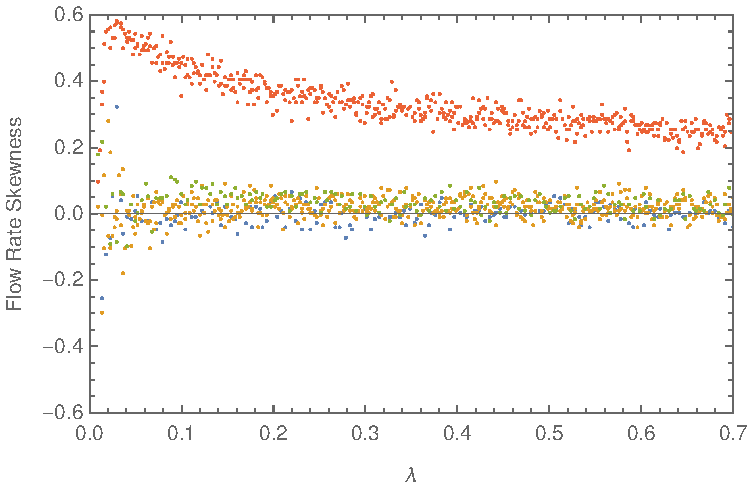
\includegraphics[width=0.5\linewidth]{../tex-src/images/lambdaScan/flowSkew} & 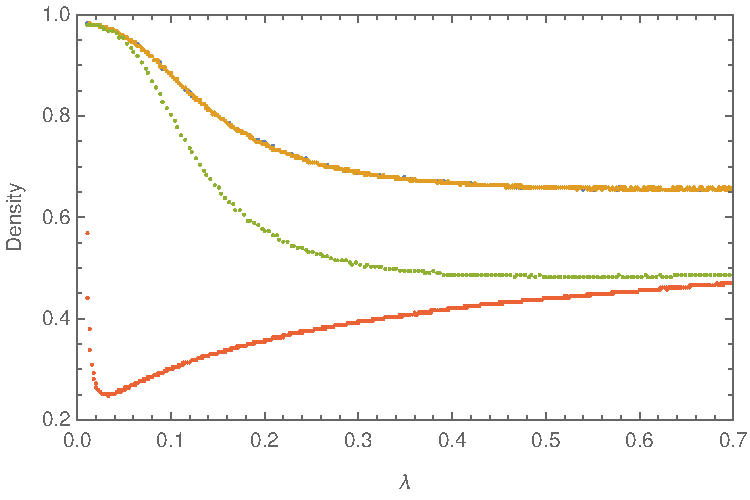
\includegraphics[width=0.5\linewidth]{../tex-src/images/lambdaScan/lambdaDens} \\
    \end{tabular}
\end{center}
    \vspace{-0em}
\end{figure*}


\subsection{Varying $\lambda$ and Boundary Densities, Keeping the Average Density Constant}
Another situation we can investigate has boundaries $(\rho_B, \rho_T) = (\rho_M + \frac{1}{2} \delta\rho, \rho_M - \frac{1}{2} \delta\rho)$ for some given $\rho_M$, where $\delta\rho$ and $\lambda$ are varied. As before, I calculated flow rate
moments and average densities, and the results are displayed in Figure~\ref{fig:constDens}. These calculations were performed with the same run parameters (system length etc)
as above.

\begin{figure*}[h!]
\vspace{1em}
\caption{\label{fig:constDens} Flow rate mean, flow variance and average overall densities observed when varying the difference $\delta\rho$ between the boundary concentrations
$(\rho_B, \rho_T) = (\rho_M + \frac{1}{2} \delta\rho, \rho_M - \frac{1}{2} \delta\rho)$ and $\lambda$. I chose $\rho_M=\frac{1}{2}$, as this gives us the biggest range of $\delta\rho$ to investigate. The top left panel is the MFT prediction
for the flow rate, whilst top right shows the observed mean flow rate. The measured flow skewness and kurtosis are not displayed here as both signals were small and noisy, and didn't show anything particularly significant.}
\begin{center}
 \begin{tabular}{c|c}
    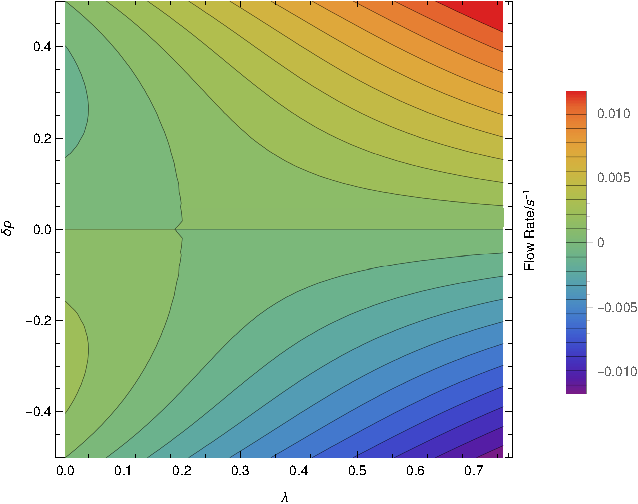
\includegraphics[width=0.5\linewidth]{../tex-src/images/constDens/constAnalFlow-crop} & 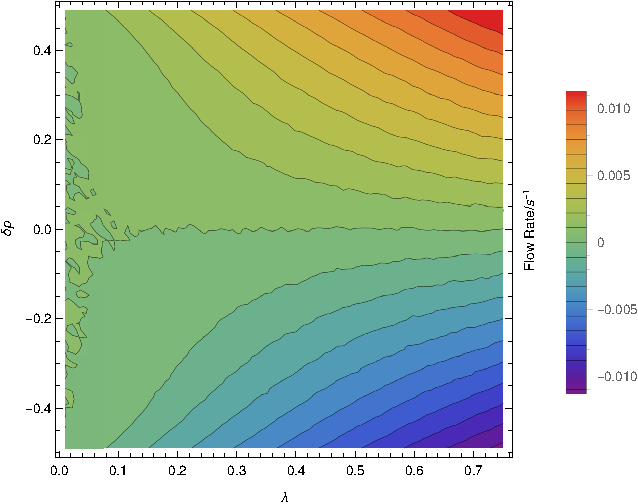
\includegraphics[width=0.5\linewidth]{../tex-src/images/constDens/meanFlowContour-crop} \\
    \hline
    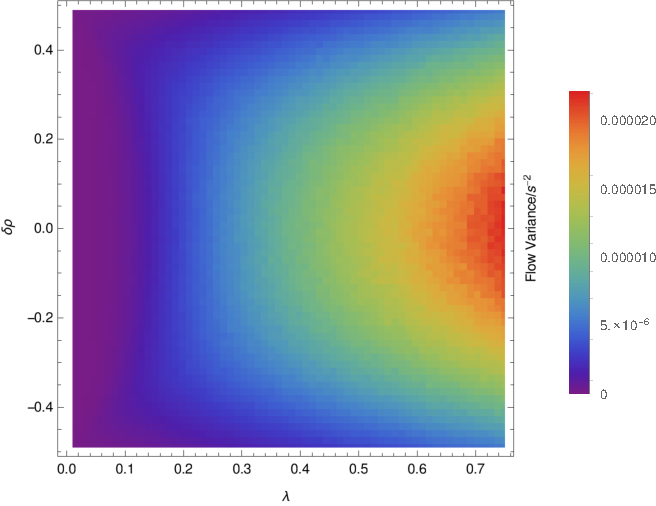
\includegraphics[width=0.5\linewidth]{../tex-src/images/constDens/varFlow-crop} & 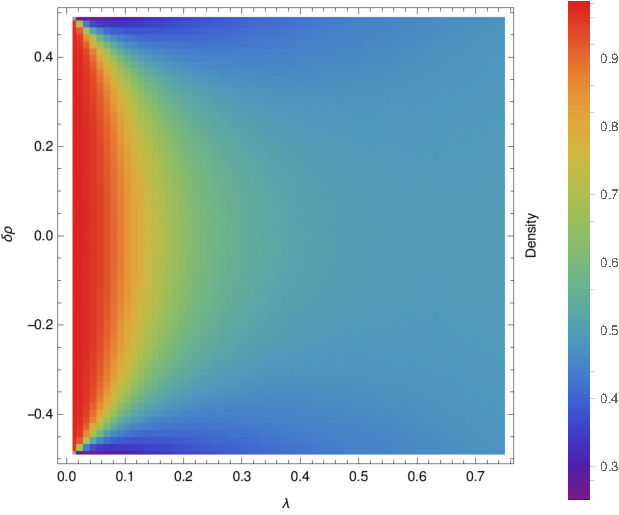
\includegraphics[width=0.5\linewidth]{../tex-src/images/constDens/meanDens-crop} \\
    \end{tabular}
\end{center}
    \vspace{-0em}
\end{figure*}



\subsection{Diffusion Coefficient Measurement}
Let us again specify the boundary densities to be $(\rho_B, \rho_T) = (\rho_M + \frac{1}{2} \delta\rho, \rho_M - \frac{1}{2} \delta\rho)$ for some given $\rho_M$. This time we keep $\delta\rho$ relatively small, so that $J$ varies approximately
linearly with $\delta\rho$; thus if we calculate $J$ for a series of small $\delta \rho$, we can perform linear regression to find $D=\partDeriv{J}{\delta\rho}\big|_{\delta\rho=0}$, the effective diffusion coefficient.
Computing this for different $(\rho_M, \lambda)$ combinations gives us numerical data which can be compared with the MFT result in Equation~\ref{eq:MFTflow}.
\begin{figure*}[h!]
\vspace{1em}
\caption{\label{fig:diffCoef} The contour plot on the left shows the MFT prediction of the diffusion coefficient $D=\partDeriv{J}{\delta\rho}\big|_{\delta\rho=0}$ as a function of local density $\rho_M$ and $\lambda$;
we are only plotting where $0 \le D \le 1.2$, other regions are shown in white, including the region in which $D<0$, which would cause instabilities and so prevent a flow from actually occurring. On the right is our numerical calculation of $D(\rho_M, \lambda)$,
with exactly the same plotting ranges. The dots indicate which points in $(\rho_M, \lambda)$ we calculated $D$ around, to give an impression of how the interpolation in the contour plot was done.}
\begin{center}
 \begin{tabular}{c@{\hspace{1em}}c}
    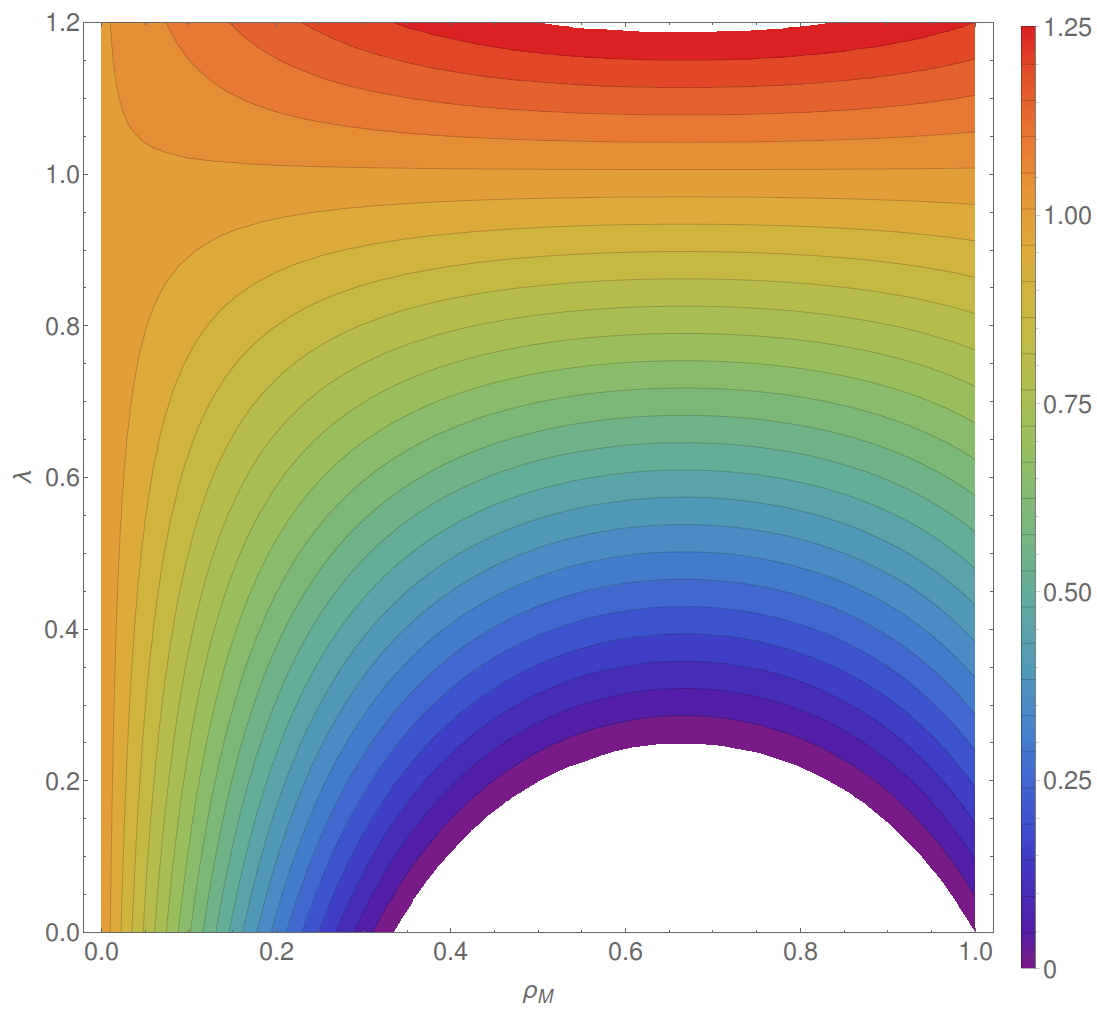
\includegraphics[width=0.5\linewidth]{../tex-src/images/analFlow.png} & 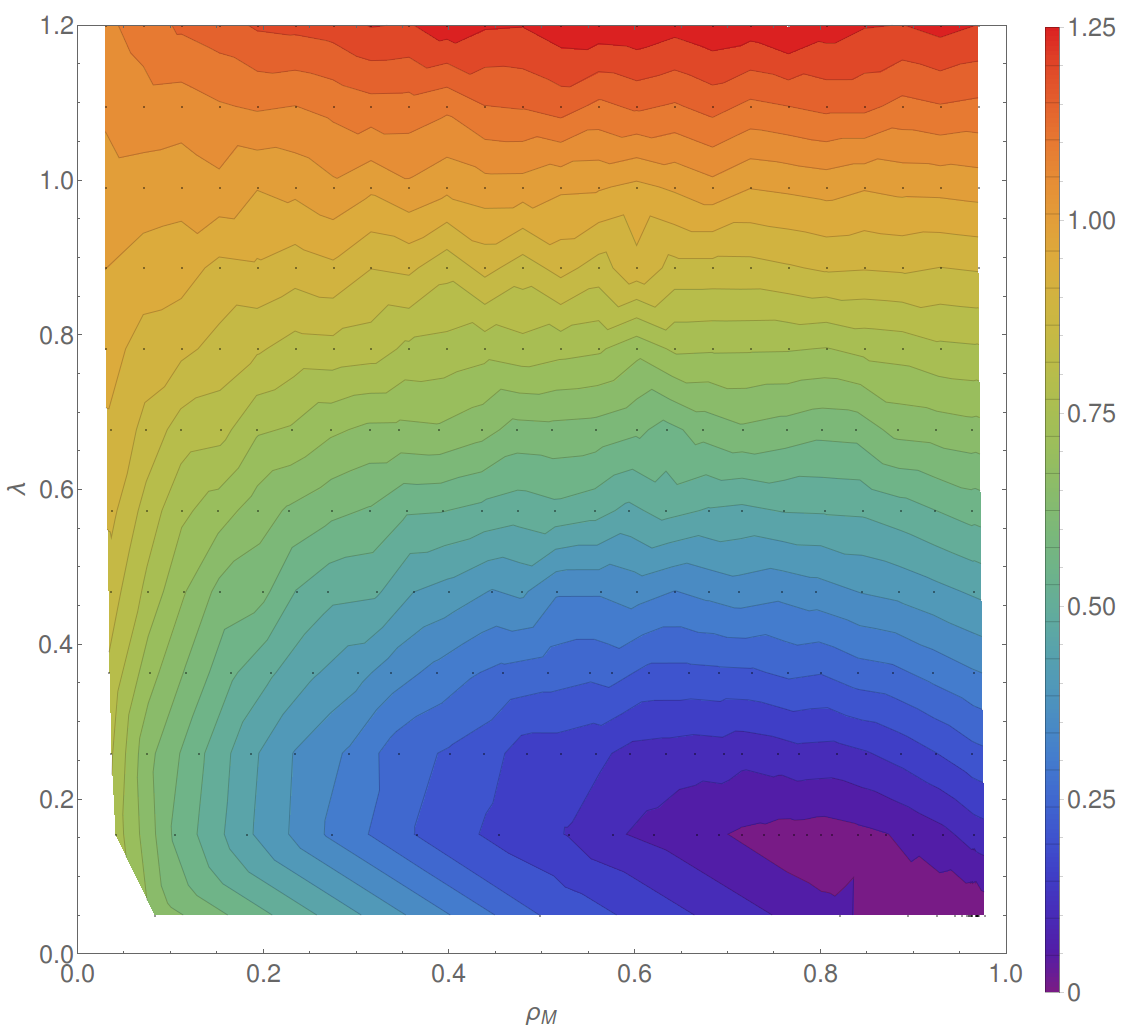
\includegraphics[width=0.5\linewidth]{../tex-src/images/dataFlow.png} \\
    \end{tabular}
\end{center}
    \vspace{-0em}
\end{figure*}
In this setup we ran the simulation for
$1.6\times10^8$ equilibration steps, followed by $10$ sets of alternating measurement and relaxation runs, of lengths $8\times10^7$ and $1.6\times10^7$ steps respectively. We repeated the calculation with a system of half the size, and again
found little difference between the two datasets, which gives us confidence that finite-size effects are small.
We can of course obtain estimates of the confidence interval for our linear regression coefficient, and thus generate a standard error for $D$; likewise we can obtain goodness of fit estimates for the
regression. They are not included here for brevity, but they are in the additional materials.
%REMEMBER TO ACTUALLY PUT IT THERE!!!

\subsection{Flow Structure}
\label{sec:flowStruc}
It is possible to produce diagrams which show the changes in short-time-averaged local density as a function of space and time. I have made such diagrams for a selection of $(\rho_M, \lambda)$ pairs, so that the reader can
get an impression of what these flows actually look like; they are shown in Figure~\ref{fig:flowPatterns}.
\iffalse
\begin{figure*}[h!]
\caption{\label{fig:flowPatterns} The spacetime flow patterns, for the $(\lambda, \rho_M)$ combinations indicated in the row and column headers. In each plot time runs along the $x$-axis, space along the $y$-axis. White represents full occupation, black empty, and grey shades partial
occupation. The degree of occupation was calculated by taking the \texttt{KMCLib} record of a particular site's occupation (i.e. the Gillespie times at
which the site changed occupation), assigning $0$ and $1$ to particles and vacancies respectively, linearly interpolating this and then integrating over times longer than a single Gillespie step but much shorter than the total time in question.
In each case the total time elapsed is that taken by $10^6$ Gillespie steps, and each short-time-average has been done over the total time divided by $508$ (to produce square diagrams, as there are $508$ active sites
per simulation). I chose to rescale time this way because if we used equal times it would appear that nothing happens in the low-$\lambda$ simulations, which isn't true!}
\begin{tabular}{c p{0.175\linewidth}}
\hspace{-2em}\begin{tabular}{c|c@{\hspace{0.25em}}c@{\hspace{0.25em}}c@{\hspace{0.25em}}c  }
  &  $\lambda=0.05$ & $\lambda=0.25$ & $\lambda=0.50$ & $\lambda=0.70$ \\ 
  \hline
   \begin{tabular}{c} \vspace{-12em} \\ \hspace{-1em}$\rho_M=0.05$\hspace{0em} \\  \\ \end{tabular} & 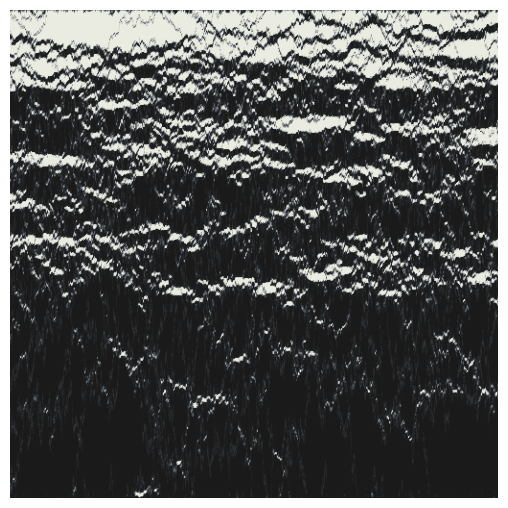
\includegraphics[width=0.24\linewidth]{../tex-src/images/flowImps/flowl0r0.png} & 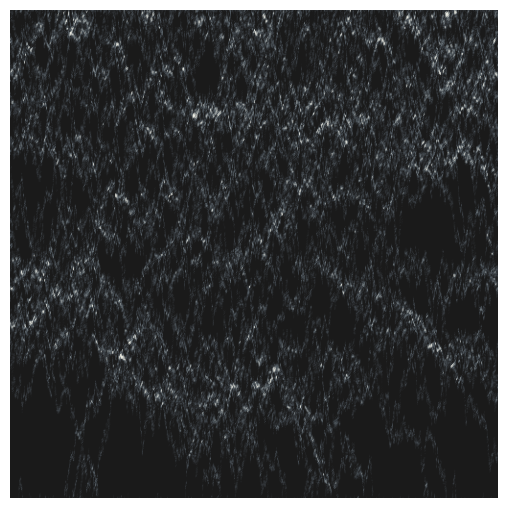
\includegraphics[width=0.24\linewidth]{../tex-src/images/flowImps/flowl1r0.png}  & 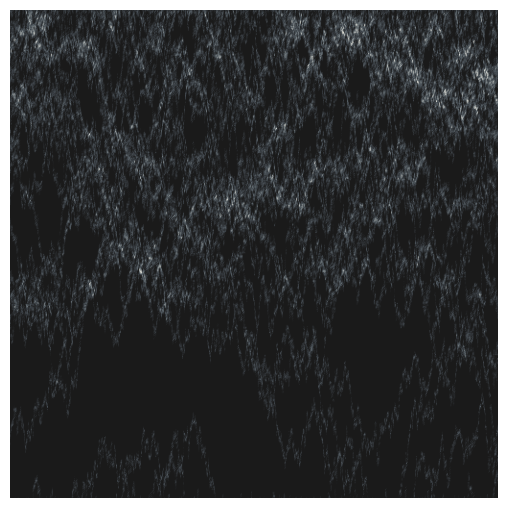
\includegraphics[width=0.24\linewidth]{../tex-src/images/flowImps/flowl2r0.png} & 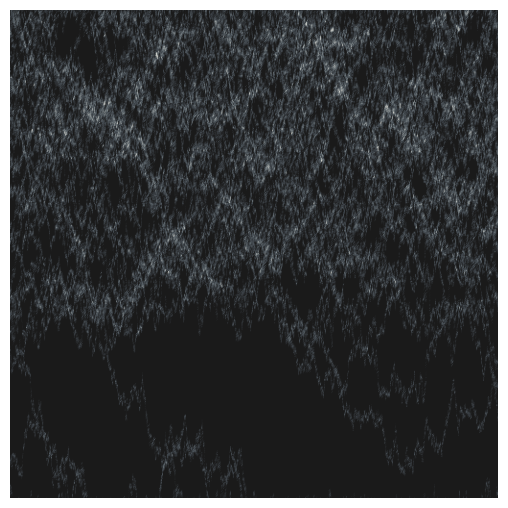
\includegraphics[width=0.24\linewidth]{../tex-src/images/flowImps/flowl3r0.png} \\
   \begin{tabular}{c} \vspace{-12em} \\ \hspace{-1em}$\rho_M=0.35$\hspace{0em} \\  \\ \end{tabular} & 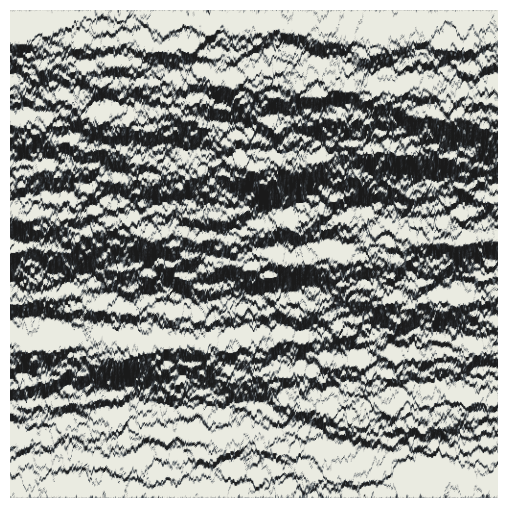
\includegraphics[width=0.24\linewidth]{../tex-src/images/flowImps/flowl0r1.png} & 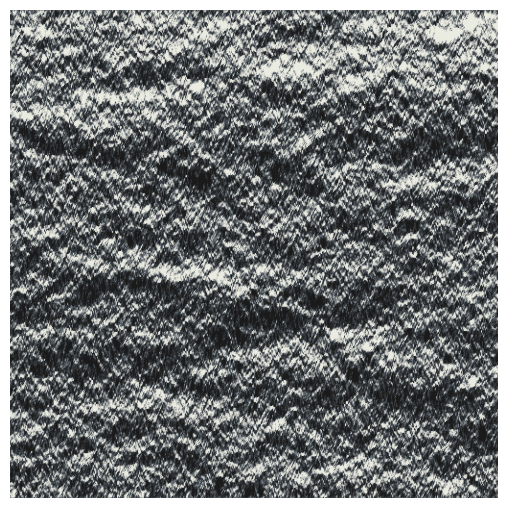
\includegraphics[width=0.24\linewidth]{../tex-src/images/flowImps/flowl1r1.png}  & 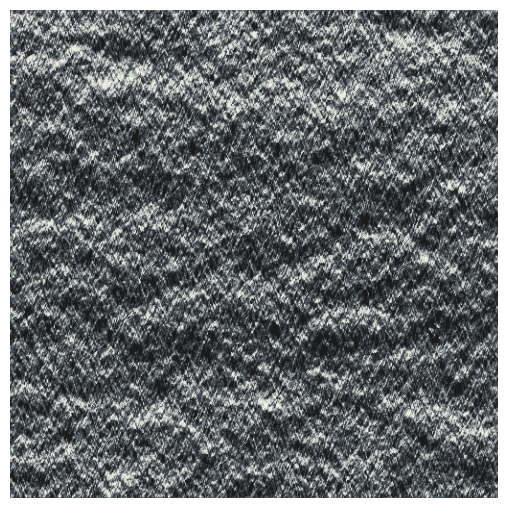
\includegraphics[width=0.24\linewidth]{../tex-src/images/flowImps/flowl2r1.png} & 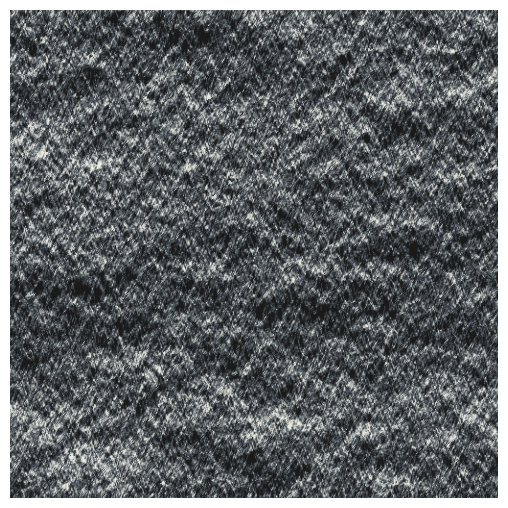
\includegraphics[width=0.24\linewidth]{../tex-src/images/flowImps/flowl3r1.png} \\
   \begin{tabular}{c} \vspace{-12em} \\ \hspace{-1em}$\rho_M=0.65$\hspace{0em} \\  \\ \end{tabular} & 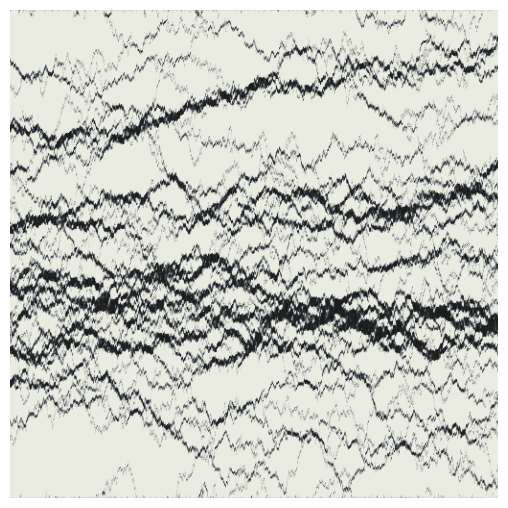
\includegraphics[width=0.24\linewidth]{../tex-src/images/flowImps/flowl0r2.png} & 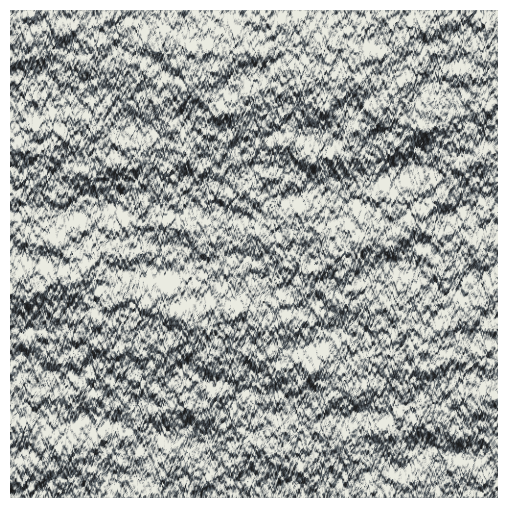
\includegraphics[width=0.24\linewidth]{../tex-src/images/flowImps/flowl1r2.png}  & 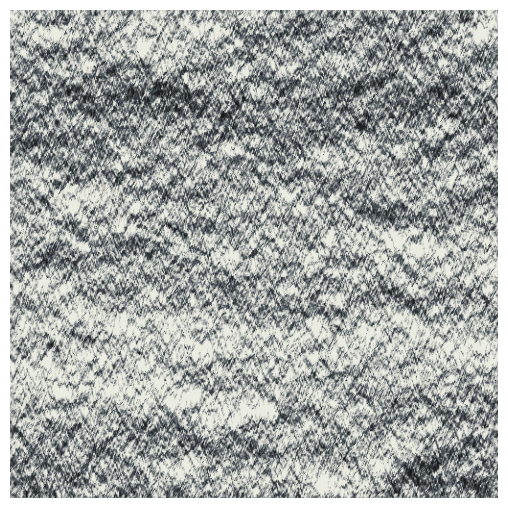
\includegraphics[width=0.24\linewidth]{../tex-src/images/flowImps/flowl2r2.png} & 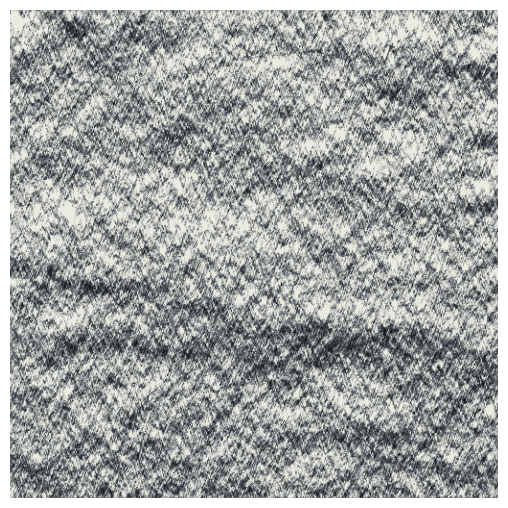
\includegraphics[width=0.24\linewidth]{../tex-src/images/flowImps/flowl3r2.png} \\
   \begin{tabular}{c} \vspace{-12em} \\ \hspace{-1em}$\rho_M=0.95$\hspace{0em} \\  \\ \end{tabular} & 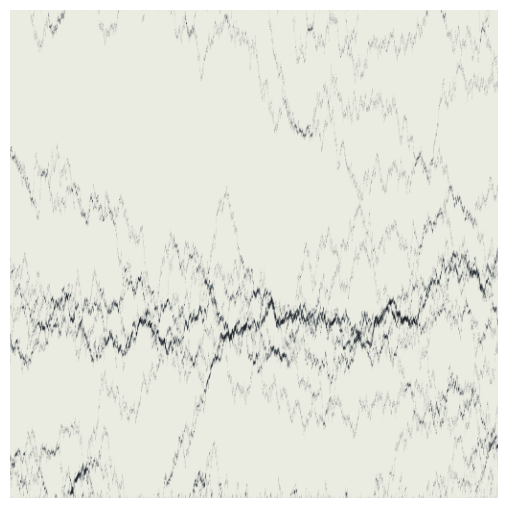
\includegraphics[width=0.24\linewidth]{../tex-src/images/flowImps/flowl0r3.png} & 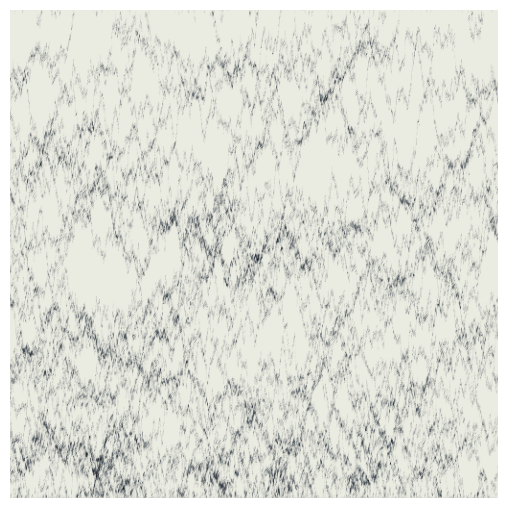
\includegraphics[width=0.24\linewidth]{../tex-src/images/flowImps/flowl1r3.png}  & 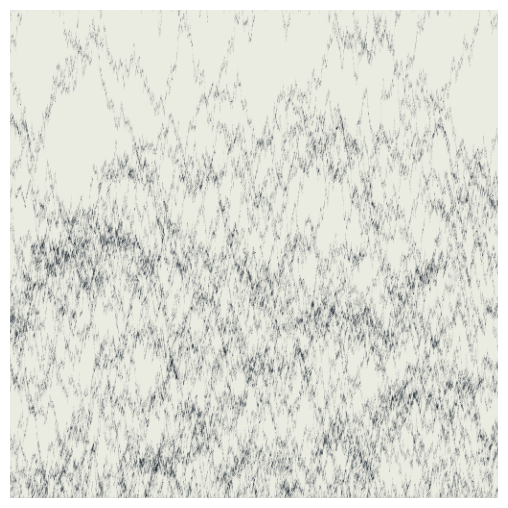
\includegraphics[width=0.24\linewidth]{../tex-src/images/flowImps/flowl2r3.png} & 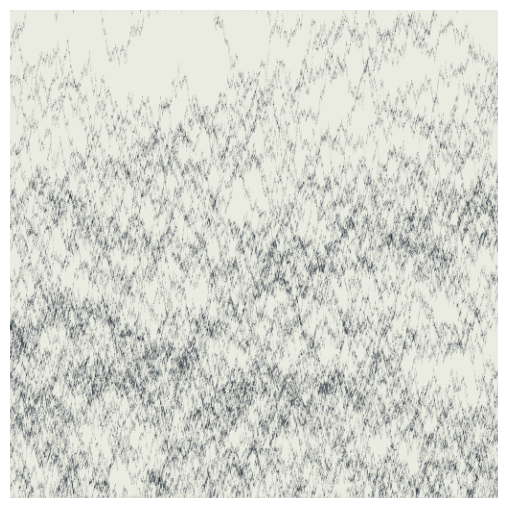
\includegraphics[width=0.24\linewidth]{../tex-src/images/flowImps/flowl3r3.png} \\
   \end{tabular}
\hspace{-1em}
&
\end{tabular}
\end{figure*}
\fi
\begin{figure*}[h!]
\caption{\label{fig:flowPatterns} The spacetime flow patterns, for the $(\lambda, \rho_M)$ combinations indicated in the row and column headers. In each plot time runs along the $x$-axis, space along the $y$-axis. White represents full occupation, black empty, and grey shades partial
occupation. The degree of occupation was calculated by taking the \texttt{KMCLib} record of a particular site's occupation (i.e. the Gillespie times at
which the site changed occupation), assigning $0$ and $1$ to particles and vacancies respectively, linearly interpolating this and then integrating over times longer than a single Gillespie step but much shorter than the total time in question.
In each case the total time elapsed is that taken by $10^6$ Gillespie steps, and each short-time-average has been done over the total time divided by $508$ (to produce square diagrams, as there are $508$ active sites
per simulation). Time has been rescaled this way in order to allow fair comparison of radically different $\lambda$-values.}
\begin{tabular}{c p{0.175\linewidth}}
\hspace{-2em}\begin{tabular}{c|c@{\hspace{0.25em}}c@{\hspace{0.25em}}c}
  &  $\lambda=0.05$ & $\lambda=0.38$ & $\lambda=1.00$ \\ 
  \hline
   \begin{tabular}{c} \vspace{-12em} \\ \hspace{-1em}$\rho_M=0.05$\hspace{0em} \\  \\ \end{tabular} & 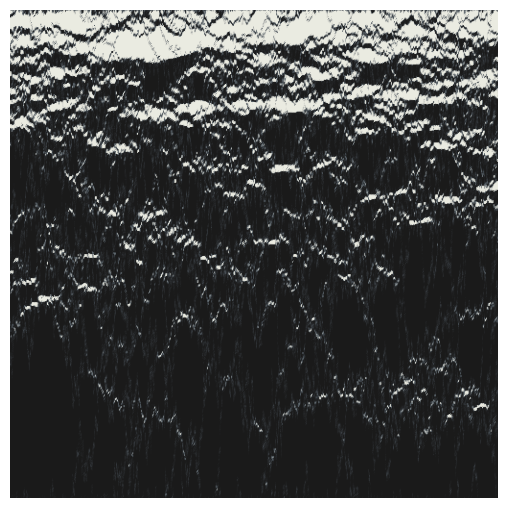
\includegraphics[width=0.32\linewidth]{../tex-src/images/flowImps2/flowl0r0.png} & 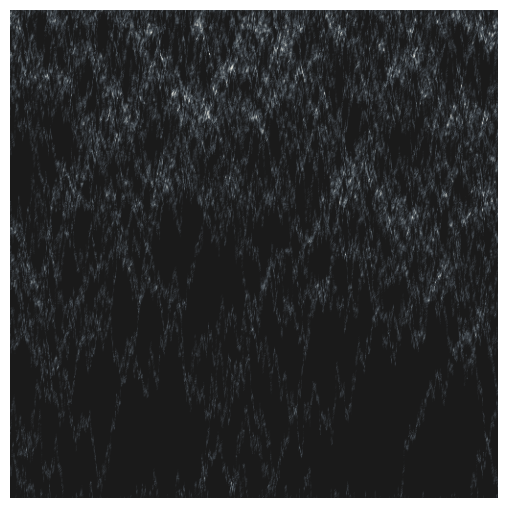
\includegraphics[width=0.32\linewidth]{../tex-src/images/flowImps2/flowl2r0.png}  & 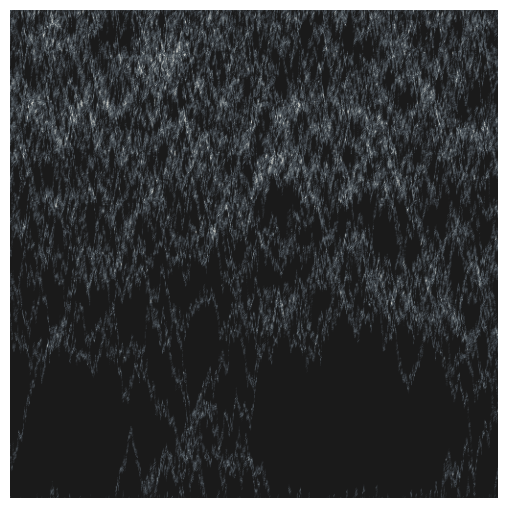
\includegraphics[width=0.32\linewidth]{../tex-src/images/flowImps3/flowl0r0.png} \\
   \begin{tabular}{c} \vspace{-12em} \\ \hspace{-1em}$\rho_M=0.50$\hspace{0em} \\  \\ \end{tabular} & 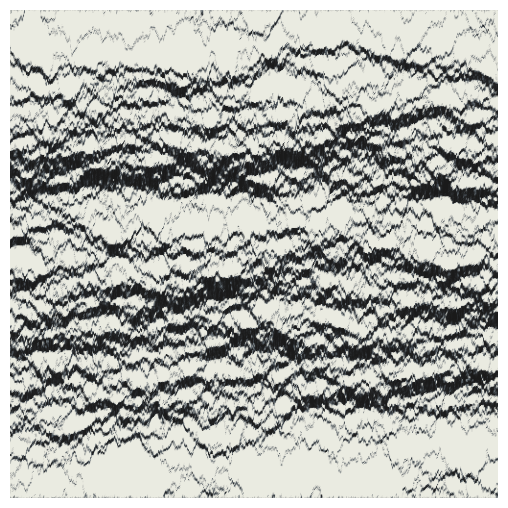
\includegraphics[width=0.32\linewidth]{../tex-src/images/flowImps2/flowl0r2.png} & 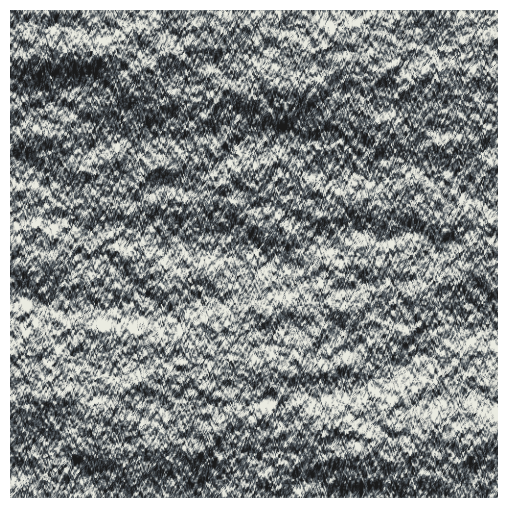
\includegraphics[width=0.32\linewidth]{../tex-src/images/flowImps2/flowl2r2.png}  & 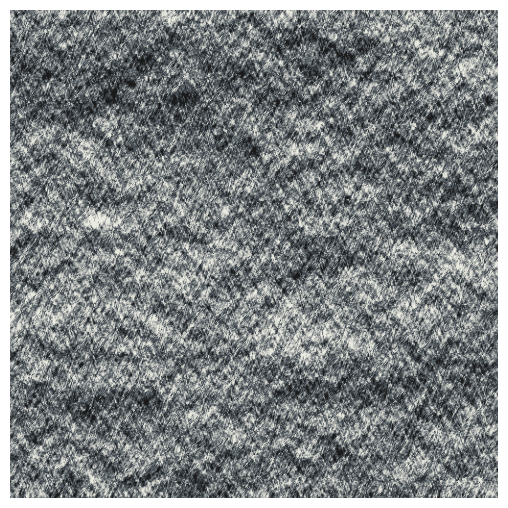
\includegraphics[width=0.32\linewidth]{../tex-src/images/flowImps3/flowl0r2.png} \\
   \begin{tabular}{c} \vspace{-12em} \\ \hspace{-1em}$\rho_M=0.95$\hspace{0em} \\  \\ \end{tabular} & 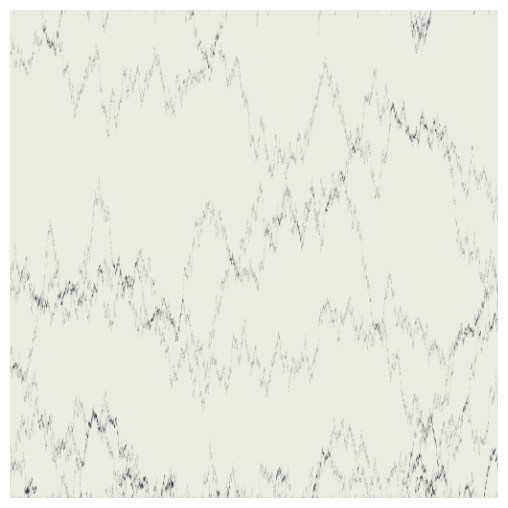
\includegraphics[width=0.32\linewidth]{../tex-src/images/flowImps2/flowl0r4.png} & 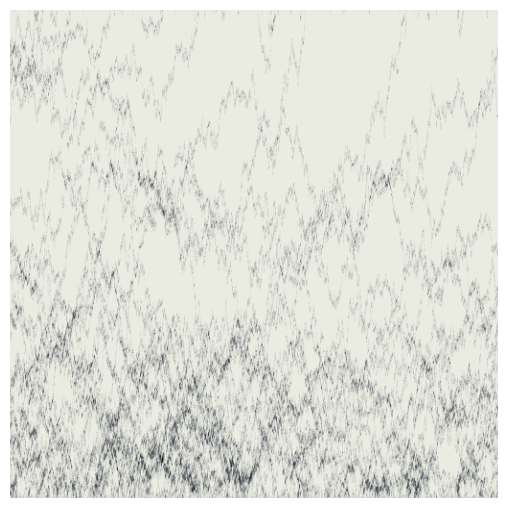
\includegraphics[width=0.32\linewidth]{../tex-src/images/flowImps2/flowl2r4.png}  & 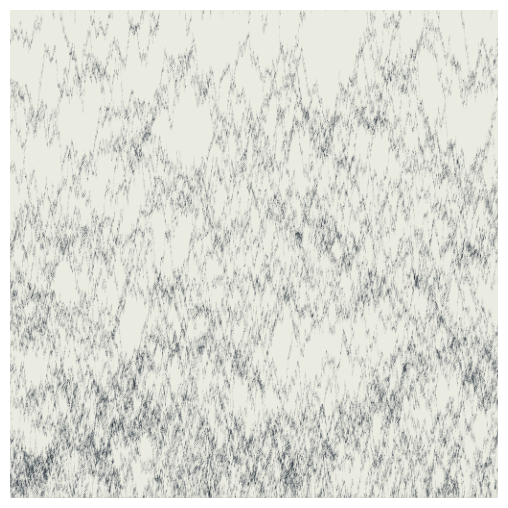
\includegraphics[width=0.32\linewidth]{../tex-src/images/flowImps3/flowl0r4.png} \\
   \end{tabular}
\hspace{-1em}
&
\end{tabular}
\end{figure*}

\iffalse
\subsection{Correlation Functions}
Whilst we're calculating flow rates, we can also use our \texttt{KMCLib} code to calculate the equal time 2-point correlation function
$C(x) = \left\langle \rho(x)\rho(0) \right\rangle - \left\langle \rho(x) \right\rangle \left\langle \rho(0) \right\rangle $.
We can calculate the same quantity in a finite periodic ring analytically, and in both the analytic and numerical cases we may attempt to extract a correlation length by (curve-fitting / Laplace transform);
hence we can check whether having a steady flow through the system causes any structural effects.}
\fi